%% 
%% Copyright 2019-2020 Elsevier Ltd
%% 
%% This file is part of the 'CAS Bundle'.
%% --------------------------------------
%% 
%% It may be distributed under the conditions of the LaTeX Project Public
%% License, either version 1.2 of this license or (at your option) any
%% later version.  The latest version of this license is in
%%    http://www.latex-project.org/lppl.txt
%% and version 1.2 or later is part of all distributions of LaTeX
%% version 1999/12/01 or later.
%% 
%% The list of all files belonging to the 'CAS Bundle' is
%% given in the file `manifest.txt'.
%% 
%% Template article for cas-sc documentclass for 
%% double column output.

% \documentclass[a4paper,fleqn,longmktitle]{cas-sc}
\documentclass[a4paper]{cas-sc}
% \documentclass{article}
% \usepackage[numbers]{natbib}
\usepackage[authoryear]{natbib}

% \usepackage[authoryear,longnamesfirst]{natbib}
% \renewcommand {\thetable} {\arabic{table}}

% \renewcommand {\thefigure} {\arabic{figure}}
\usepackage{chngcntr}%需要调用这个宏包
\counterwithout{figure}{section}%
\usepackage{threeparttable}
% \usepackage[section]{placeins}
\usepackage{afterpage}
% \usepackage[disable]{endfloat}
\usepackage{amsmath}
\usepackage{ntheorem}
\newtheorem{theorem}{Theorem}
\newtheorem{lemma}[theorem]{Lemma}
\newtheorem*{proof}{Proof}
\newtheorem{remark}[theorem]{Remark}
\newtheorem{defi}[theorem]{Definition}
\newtheorem{property}[theorem]{Property}
\newtheorem{corollary}[theorem]{Corollary}
%%%Author definitions
\def\tsc#1{\csdef{#1}{\textsc{\lowercase{#1}}\xspace}}
\tsc{WGM}
\tsc{QE}
\tsc{EP}
\tsc{PMS}
\tsc{BEC}
\tsc{DE}
%%%

% Uncomment and use as if needed
%\newtheorem{theorem}{Theorem}
%\newtheorem{lemma}[theorem]{Lemma}
%\newdefinition{rmk}{Remark}
%\newproof{pf}{Proof}
%\newproof{pot}{Proof of Theorem \ref{thm}}

\begin{document}
\let\WriteBookmarks\relax
\def\floatpagepagefraction{1}
\def\textpagefraction{.001}


% Short author
\shortauthors{Tiancheng Ruan et~al.}
\shorttitle{}

% Main title of the paper
\title [mode = title]{123123}
% Title footnote mark
% eg: \tnotemark[1]
% \tnotemark[1,2]

% Title footnote 1.
% eg: \tnotetext[1]{Title footnote text}
% \tnotetext[<tnote number>]{<tnote text>} 
% \tnotetext[1]{This document is the results of the research
%    project funded by the National Science Foundation.}

% \tnotetext[2]{The second title footnote which is a longer text matter
%    to fill through the whole text width and overflow into
%    another line in the footnotes area of the first page.}


% First author
%
% Options: Use if required
% eg: \author[1,3]{Author Name}[type=editor,
%       style=chinese,
%       auid=000,
%       bioid=1,
%       prefix=Sir,
%       orcid=0000-0000-0000-0000,
%       facebook=<facebook id>,
%       twitter=<twitter id>,
%       linkedin=<linkedin id>,
%       gplus=<gplus id>]
\author[1,2,3]{Tiancheng Ruan}[style=chinese]
\ead{ruantiancheng@seu.edu.cn}
\credit{Conceptualization of this study, Methodology,Writing - Original draft preparation,Resources, Software}

\author[1,2,3]{Hao Wang}[style=chinese]
% Corresponding author indication
\cormark[1]

% % Footnote of the first author
% \fnmark[1]

% Email id of the first author
\ead{haowang@seu.edu.cn}

% % URL of the first author
% \ead[url]{www.cvr.cc, cvr@sayahna.org}

%  Credit authorship
\credit{ Formal analysis,Funding acquisition,Supervision,Writing - review \& editing}

% Address/affiliation
\affiliation[1]{organization={Jiangsu Key Laboratory of Urban ITS, Southeast University},
  addressline={2 Si Pai Lou},
  city={Nanjing},
  % citysep={}, % Uncomment if no comma needed between city and postcode
  postcode={210096},
  % state={},
  country={P.R. China}}

\affiliation[2]{organization={Jiangsu Province Collaborative Innovation Center of Modern Urban Traffic Technologies},
  addressline={2 Si Pai Lou},
  city={Nanjing},
  % citysep={}, % Uncomment if no comma needed between city and postcode
  postcode={210096},
  % state={},
  country={P.R. China}}
\affiliation[3]{organization={School of Transportation, Southeast University},
  addressline={2 Si Pai Lou},
  city={Nanjing},
  % citysep={}, % Uncomment if no comma needed between city and postcode
  postcode={210096},
  % state={},
  country={P.R. China}}
% Second author


% Third author
\author[1,2,3]{Linjie Zhou}[style=chinese]
% \fnmark[2]
\ead{220193107@seu.edu.cn}
% \ead[URL]{www.sayahna.org}
\credit{Data curation,Investigation}



% Fourth author
% \author%
% [4]

\author[1,2,3]{Gengyue han}[style=chinese]
% \fnmark[2]
\ead{gyhan@seu.edu.cn}
% \ead[URL]{www.sayahna.org}
\credit{Writing - Original draft preparation}

\author[1,2,3]{Beier Ba}[style=chinese]
% \fnmark[2]
\ead{980794728@qq.com}
% \ead[URL]{www.sayahna.org}
\credit{ Formal analysis, Writing - Original draft preparation}

\author[1,2,3]{Changyin Dong}[style=chinese]
% \fnmark[2]
\ead{dongcy@seu.edu.cn}
% \ead[URL]{www.sayahna.org}
\credit{Formal analysis,Funding acquisition}
% \affiliation[4]{organization={MOE Key Laboratory for UrbanTransportation Complex Systems Theory and Technology, Beijing Jiaotong University},
%     city={Beijing},
%     % citysep={}, % Uncomment if no comma needed between city and postcode
%     postcode={100044}, 
%     % state={},
%     country={P.R. China}}
% \affiliation[5]{organizati on={State Key Laboratory of Fire Science and School of Engineering Science, University of Science and Technology of China},
%     city={Hefei},
%     % citysep={}, % Uncomment if no comma needed between city and postcode
%     postcode={230026}, 
%     % state={},
%     country={P.R. China}}



% Corresponding author text
\cortext[cor1]{Corresponding author}

% Footnote text
% \fntext[fn1]{This is the first author footnote. but is common to third
%   author as well.}
% \fntext[fn2]{Another author footnote, this is a very long footnote and
%   it should be a really long footnote. But this footnote is not yet
%   sufficiently long enough to make two lines of footnote text.}

% For a title note without a number/mark
% \nonumnote{This note has no numbers. In this work we demonstrate $a_b$
%   the formation Y\_1 of a new type of polariton on the interface
%   between a cuprous oxide slab and a polystyrene micro-sphere placed
%   on the slab.
%   }

% Here goes the abstract
\begin{abstract}
  12312
\end{abstract}

% Use if graphical abstract is present
% \begin{graphicalabstract}
% 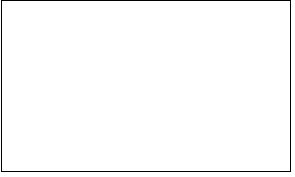
\includegraphics{figs/grabs.pdf}
% \end{graphicalabstract}

% Research highlights
\begin{highlights}

  \item 123
\end{highlights}

% Keywords
% Each keyword is seperated by \sep
\begin{keywords}
  123 \sep 1231
\end{keywords}


\maketitle

\section{Introduction}
\label{Section 1}
123\citep{Gu2003}

\section{Preliminaries}
\label{Section 2}
123
\subsection{Network model}
\label{Section 2.1}
123
\section{System modeling}
\label{Section 3}
123
% \begin{figure}
%   \centering

%   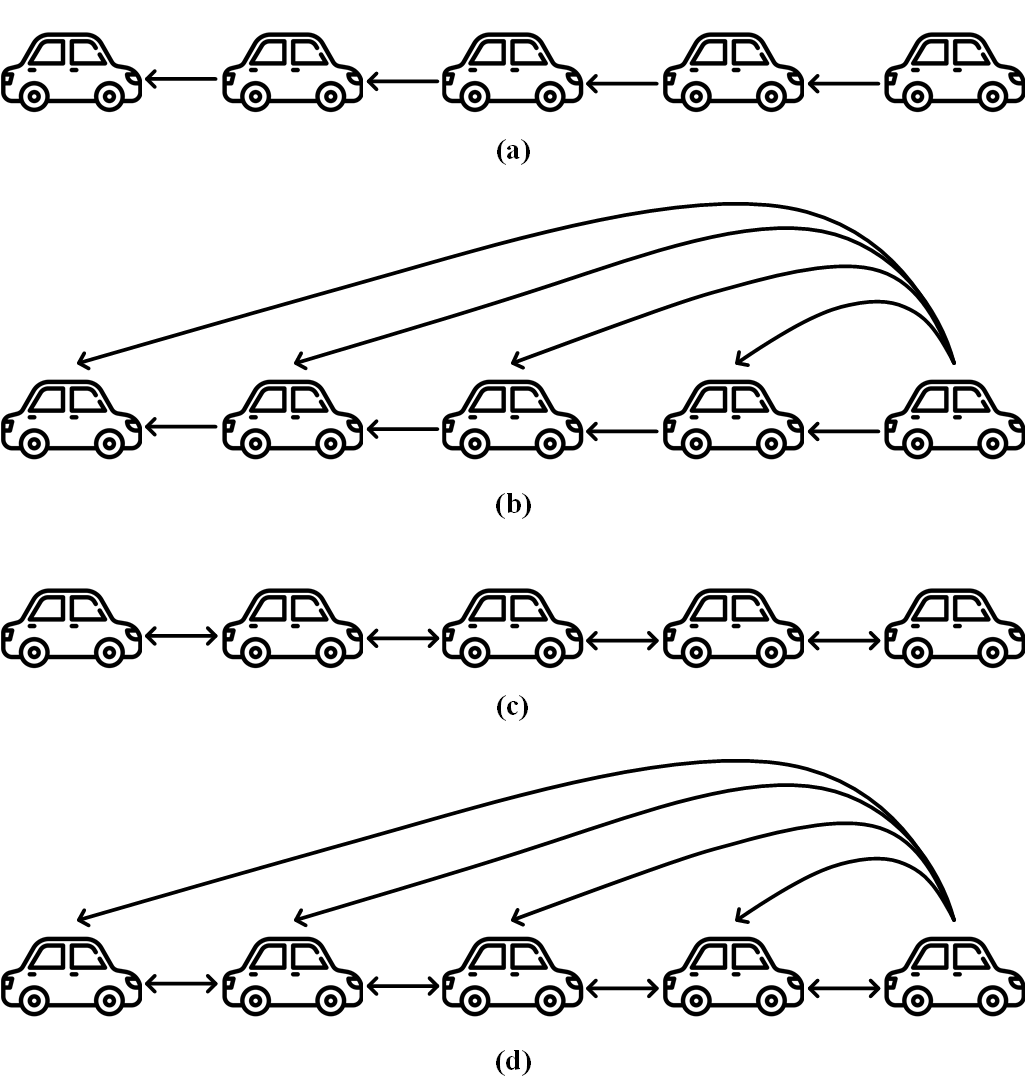
\includegraphics[width=14cm]{figs/fig1.png}
%   \caption{~.}
%   \label{fig1}
% \end{figure}

\subsection{Vehicle longitudinal dynamic Modeling}
\label{Section 3.1}
123


\section{Stability analyses}
\label{Section 4}
123
\section{Numerical analyses}
\label{Section 5}
123
% \begin{table}
%   \centering
%   \setlength{\abovecaptionskip}{0pt}
%   \setlength{\belowcaptionskip}{10pt}%设置标题与表格的距离
%   \begin{threeparttable}[b]

%     \caption{~Network and traffic simulation parameters.}
%     \label{table1}
%     {\begin{tabular}{lc} \toprule
%         Parameters                                         & Value               \\ \midrule
%         Platoon size $n$                                   & 5 vehicles          \\
%         \bottomrule
%       \end{tabular}}
%     \begin{tablenotes}
%       \item[1] \citep{Wang2018a,Zhou2020}
%     \end{tablenotes}
%   \end{threeparttable}
% \end{table}


\section{Conclusion and future work}
\label{Section 6}
123
\appendix


\section*{Appendix A.~Feedback control for linearization}
\label{AppendixA}
123

\printcredits

\section*{Acknowledgment}

This research was sponsored by the National Science Foundation of China (No. 51878161 and No.52072067), Postgraduate Research \& Practice Innovation Program of Jiangsu Province (KYCX22\_0266).

%% Loading bibliography style file
% \bibliographystyle{model1-num-names}
\bibliographystyle{cas-model2-names}

% Loading bibliography database
\bibliography{cas-refs}


%\vskip3pt

\end{document}

